\documentclass[12pt]{article}
\usepackage{graphicx}
\usepackage{amsmath}
\usepackage{float}
\title{Lab 1: Rainy Analog Days}
\author{Xin Gao}
\date{\today}

\begin{document}
\maketitle
\section{Abstract}
Construction of FM D demodulator (radio receiver) for receiving radio signals and of an
amplifier for increasing such signals begin with certain circuit - RC
filters (high and low pass), RLC bandpass filter, transistor, and
rectifier are used for the constructions. The FM demodulator produced
expected results of only certain frequencies levels at the output. The
amplifier produced gains at the output. Mathematical modeling of the
thermal noise within the receiver-amplifier are used in the context of
internal thermal noise. Its seemingly random distribution approach a
Gaussian behavior at large samples, which also lead to decreasing mean
standard deviation. 


\section{Introduction}
Applying foundational knowledge of electronics and
mathematical physics, one can, from the breadboard up in the lab, create devices such a
frequency-modulated (FM) radio receiver or a speaker amplifier. Simple
systems such as filters and transistors can combine to make more
complex systems that are used in many areas in the technical
world. Through these simple experiments, the intricacies of the physical
workings of electronic devices are explored. More fundamentally, the
underlying math behind statistical phenomena in physics such as random noise
distributions are explored and explained. In the end, from one wire
to the next, everything seems connected.

\section{Methods and Procedure}
Experiments and observations are carried out primarily in three
distinct parts: the construction of the FM radio receiver and its
associated circuits; the construction of the speaker amplifier; and the
measurement on the noise figure of the amplifier.

\subsection{Important Equations and Terms}
\begin{itemize}
\item Voltage (V): usually the output, as a function of frequency, of a
  signal. It is often associated with the amplitude of the signal.
\item Impedance (Z): replaces resistance in the generalized Ohm's Law. While
  resistors have resistance, capacitors and inductors have
  reactance. They are given by
\begin{align}Z_{C} = \frac{1}{i\omega{C}}\,\,\,\,\,\,\,\,\, Z_{L} =
  i\omega{L}\end{align}
Here, i is the imaginary number and $\omega = 2\pi{f}$.
\item Ohm's Law: $V = IZ$ where I is the current.
\item The ratio of output voltage to input voltage can be generalized to
\begin{align}\frac{V_{out}}{V_{in}} = \frac{Z_{2}}{Z_{1} +
    Z_{2}}\end{align}
This equation arise from measuring the output voltage of a voltage
divider circuit.  $Z_{1}$ and $Z_{2}$ are anything with impedance in series.
\end{itemize}

\subsection{FM Demodulation}
The FM radio receiver is broken down into several multi-unit
core components: A resistor-inductor-capacitor(RLC) filter; a voltage
biaser; a high-pass filter; and coupling and decoupling capacitors. See
figure 1.
\begin{figure}[H]
\centering
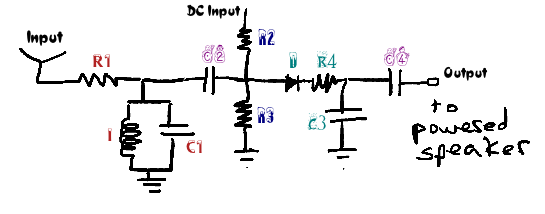
\includegraphics[width=.9\textwidth]{fm_demodulation.png}
\caption{FM Demodulator with its resistors(R), capacitors(C), diode(D) and
  inductor(L) labelel and colored according to its function in
  the circuit. Red is the LC circuit; violet are the coupling or
  decoupling capacitors; torqoise is the high pass filter; and blue is
  the biaser.}
\end{figure}
\subsubsection{RLC Circuit}
After the signal enters the circuit via the input, it first encounters
the RLC circuit, composed of $R_{1}$, L, and $C_{1}$. The purpose of the RLC
filter is to allow only 1 certain band of frequency to pass through. At frequency $f_{0}$ set by the
signal and with specific values for $R_{1}$, L, and $C_{1}$, the output has a peak
value or near 1 output to input voltage ratio with a narrow band of voltage spike around it. The
equation relating the variables is:

\begin{align} \frac{f_{0}}{(\Delta{f_{-3dB}})} =
  \omega_{0}RC\end{align}
Here $f_{0}$ is the resonant frequency; it is where the output
($V_{out}/V_{in}$) peaks. It equals $1/2\pi{sqrt{LC}}$. $\omega_{0}$ is
equivalent to $1/sqrt{LC}$. The width of the band is approximately
$\Delta{f_{-3dB}}$ with dB meaning decibels. This expression means 
``the difference in values of frequencies at which the
output voltage to input voltage returns -3 decibels.'' The decibels
equation is logarithmic: dB = $10\log_{10} V_{out}/V_{in}$. At input
signal frequency of 1.045 MHz and given the band width of 200 kHz, the
values chosen for $R_{1}$, $C_{1}$ and I are 234 $\Omega$, $1\times{10^{-8}}$
F, and $2\times{10^{-8}}$ H respectively. Using the voltage divider
equation and manipulate it for this case, the resulting equation
relating $V_{out}/V_{in}$ to frequency is:
\begin{align}\frac{V_{out}}{V_{in}} =
  \frac{\omega{L}}{R\|{\omega}^{2}{LC} - 1\| + \omega{L}}\end{align}
\begin{figure}[H]
\centering
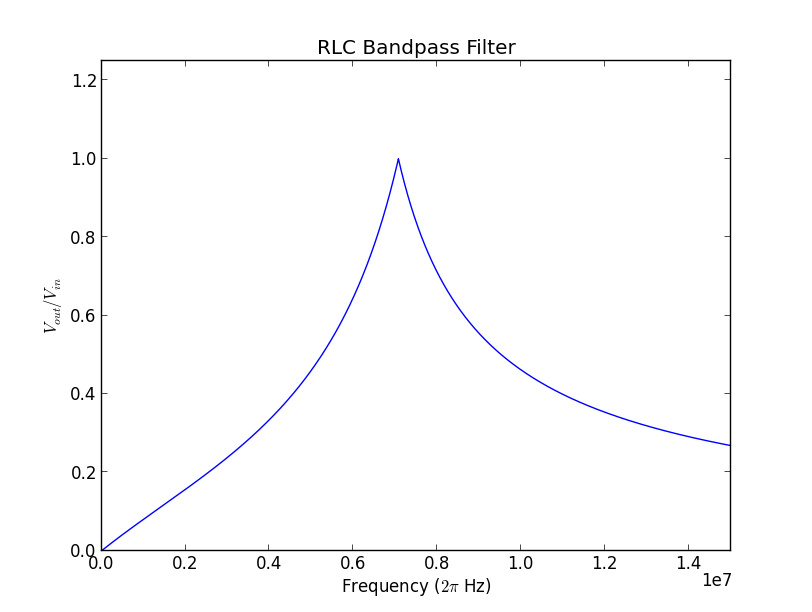
\includegraphics[width=.95\textwidth]{RLC_filter.png}
\caption{Output to input voltage ratio shown as a function of angular
  frequency $\omega$ ($2\pi{f}$). At the peak, $\omega$ is approximately
  7 MHz (so f is approximately 1 MHz).} 
\end{figure}
We measure at a frequency slightly higher than the peak frequency to
avoid a measurement that can possible blow up at the peak
frequency. Measuring it in the band allows us to still see a significant
increase in the ratio while avoiding unnecessary complications.

\subsubsection{Voltage Biaser}]
$R_{2}$ and $R_{3}$ are the resistors manipulating, or biasing, the
voltage coming into or going out of the circuit. These two resistors are
in series so their combined value influence the amount of current
flowing into the diode from the DC voltage source, which is used to
increase the voltage in the circuit after the voltage has been reduced
by the RLC circuit. A current in the mA range should produce a forward
voltage drop (from anode to cathode). A total resistor value of about
2000 $\Omega$ should provide a good current amount (~0.7 25 mA) for the
diode, resulting in a ~0.7 voltage drop across the diode. Before going
into the diode, the incoming signal is a superposition of the
RLC-filtered AC signal and the DC signal.

\subsubsection{Low-Pass Filter with Diode}
D is the diode while $R_{3}$ and $C_{3}$ make up the low-pass
filter. The diode acts as a rectifier; that is, its goal is to convert
AC signals to DC signals so that the low pass filter with have an easy
time interpreting the incoming voltage values (an AC signal will be
difficult to decipher as it alternates to negative values). The low pass
filter allows low frequencies to pass while inhibiting high
frequencies. The cutoff frequency is given by:
\begin{align} f = \frac{1}{2\pi{RC}} \end{align}
For f = 100 kHz, below which would typically be considered low
frequencies for such purposes, resistor and capacitor values of about
160 $\Omega$ and $1\times{10^{-8}}$ should give the approriate
impedance. 

\subsubsection{Coupling and Decoupling Capacitors}
The purpose of $C_{2}$ is to decouple the signal: it removes the carrier
signal from the original source and leaves up with only our filtered
signal. $C_{4}$ is a coupling capacitor. Now that our signal has been
filtered by a low pass filter as a DC signal, we would want an AC output
so that we can read it on the oscilloscope. The couping capacitor return
the original AC signal.

\subsection{Speaker Amplifer}
It is possible to amplify an incoming signal using an amplifier
circuit. A BJT amplifer consists of a high pass filter, a transistor,
and several resistors.
\begin{figure}[H]
\centering
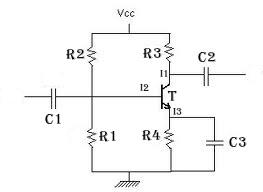
\includegraphics[width=.75\textwidth]{amplifier.png}
\caption{An amplifier. ``I'' denotes the current and T marks the
  transistor. The input comes from the left and $V_{CC}$ is an
  additional voltage source. $I_{C}$ is to be equal to $I_{E}$.}
\end{figure}
Here $C_{1}$ and $R_{2}$ together functions as a high pass
filter. $R_{1}$ and $R_{2}$ are the resistors used to set a bias voltage
into the base of the transistor. $R_{3}$ And $R_{4}$ are there to crease
a bias current. The remaining capacitor are used for additional coupling
purposes.

\subsubsection{Transistor}
The transistor consists of three parts: The base, emitter, and
collector. The purposes of a transistor is to act as a ``switch'' that
determines when a current should continue to flow through the circuit. 
The base receives incoming current and a voltage is applied
across the transistor to the emitter, $V_{BE}$. $V_{BE}$ must be around
0.6 V or higher for our transistor to continue to allow current to
flow. If $V_{BE}$ is less than 0.6 V, meaning that the outgoing voltage
from the transistor is approaching the incoming value, then the
transistor will cease to allow currents to pass. If $V_{BE}$ is
significantly above 0.6 V, then the collector will send currents to
increase the outgoing voltage. Typically, at least $V_{CE} = 0.2 V$ is
required for such a reaction to occur. The transistor thus acts to hold
the voltage constant at its separation point of the circuit. For our
purposes, let the desired voltage at $V_{out}$ = 2.5 V.
\subsubsection{Bias Current and Gain}
The gain is the ratio of the desired amplification of the output
voltage. It is also the ratio of the resistance values of $R_{3}$ and
$R{4}$ since these resistors determine the amount of gain that will
occur at the output. Taking the voltage at $V_{out}$ at 2.5, and the
incoming additional voltage at 5 V, we use Ohm's Law at $R_{3}$ to
determine $I_{C}$. With $R_{3}$ = 1000 $\Omega$, we get $I_{C}$ = 8.3 mA. Since
$I_{C} = I_{E}$, to maintain a gain of 5, the resistor values have to
maintain that ratio. We thus choose $R_{4}$ to be 200 $\Omega$. With
these value, the voltage at the emitter is approximately 0.3 V.

\subsubsection{High Pass Filter}
Our high pass filter consists of $C_{1}$ and $R_{2}$. Using the equation
$f=1/2\pi{RC}$ and the given signal frequency value of 10 kHz, we use a
$1 * 10^{-6}$ F capacitor with a 16 $\Omega$ resistor. This filter
allows most frequencies above 10 kHz to pass while denying most of lower
frequencies. This circuit allows for many different bands of frequencies
to be used for the signal. Since frequency is related to the impedance
values chosen here, adjusting the values of this amplifer circuit will
allow different frequency ranges to pass through it. 

\subsubsection{Bias Voltage}
$R_{1}$ and $R_{2}$ constitute the part of that circuit that sets a
voltage bias at the base. Since the voltage the emitter is around 0.3 V, we want our
voltage at the base $V_{B}$ around 1 V, a 4 V drop from $V_{CC}$ = 5.
We determine the value of $R_{1}$ by using this method:
\begin{align}\frac{V_{B}}{V_{CC}} = \frac{1}{5} = \frac{R_{2}}{R_{1} +
    R_{2}}\end{align}
We see that the value $R_{1}$ is four times that of $R_{2}$. Since we
have $R_{2}$ as 16 $\Omega$, we use 64 $\Omega$ for $R_{1}$. Now the
voltage difference between the base and emitter is $V_{BE}$ = 0.7.
\subsubsection{Input and Output Impedance}
The input impedance can be obtained when the transistor is ``switched
off'.'' When $V_{BE}$ is quite below 0.7, the transistor stops the
current flow so the path the input signal takes is through $R_{2}$ and
$R_{4}$. The input impedance $Z_{in}$ is then $16 \Omega + 200 \Omega = 216
\Omega$. The output impedance is obtained when the switch is on. In this
case, the current passes through all 4 resistors so $Z_{out}$ is 200 +
1000 + 64 + 16 = 1280 $\Omega$, which is bigger than $Z_{in}$ by about a
factor of 6.
\subsubsection{Termination}
It's possible that the amplifier is connected to a speaker via long
cable cord. Let's assume that the speaker inherently has 8 $\Omega$
resistance. In order for your output signal to reach the speaker
smoothly, your cable should also have a resistance of 8 $\Omega$;
otherwise, part of the signal will reflect back. With matching
impedances, the signal will think the speaker is a continuation of the
wire and will proceed into the speaker. 

\subsection{Noise}
Noise is usually unintended or undesired current due to the random
motion of electrons in objects such as a resistor. Because electrons are
omnipresent, nearly everything has some inherent noise that must be
accounted for when making precise measurements. The resulting motion of
the electrons also creates additional temperature within the object.
\subsubsection{Determining the Noise Figure}
A noise figure is a measure of the ratio of output signal power to the
noise power generated internally by thermal noise. To determine the
noise figure of a system (in our case a signal receiver), first calculate the
temperature of a resistor by using an input voltage; specifically, we
are looking for a power value, which can be obtained with P = IV. The
relationship between power and resistance is given by the
Stefan-Boltzmann Law:
\begin{align}P = A\sigma{\epsilon{T^4)}}\end{align}
Here T is temperature, A is the cross-sectional area of the object in
question, $\sigma$ is the stefan-boltzmann constant, and $\epsilon$ is
the emissivity constant which has a maximum value of 1, depending on how
much of a blackbody the object is, thus setting a
lower-bound limit of the value  of temperature given power. For our purposes, we input
a power value of 2 watts into a 50 $\Omega$ resistor. Since other terms
are constants, we can obtain the temperature of the resistor. For
convenience, we can obtain the gain required to view the noise level of
the resistor by amplyfing the noise signal until an output becomes
decipherable on an oscilloscope. With the resistor temperature in mind,
we now proceed to calculating our noise figure. Back to our receiver,
we measure its output power. Plugging that value into the
Stefan-Boltzmann Law returns the temperature of the system. Accounting
for our resistor temperature, we now have the receiver temperature. 
\subsubsection{Central Limit Demonstration}
Access my repository:
\begin{itemize}
\item https://github.com/rgao/lab\_analog\end{itemize}
The central limit theorem states that as the number of random samples
approach infinity, then the distribution becomes Gaussian with a 0
mean and 1 variance. This leads to two results:
\begin{itemize}
\item The variance of the sum is the sum of the variance of random samples.
\item Normal (Gaussian) distributions occur everywhere in nature.\end{itemize}
\begin{figure}[H]
\centering
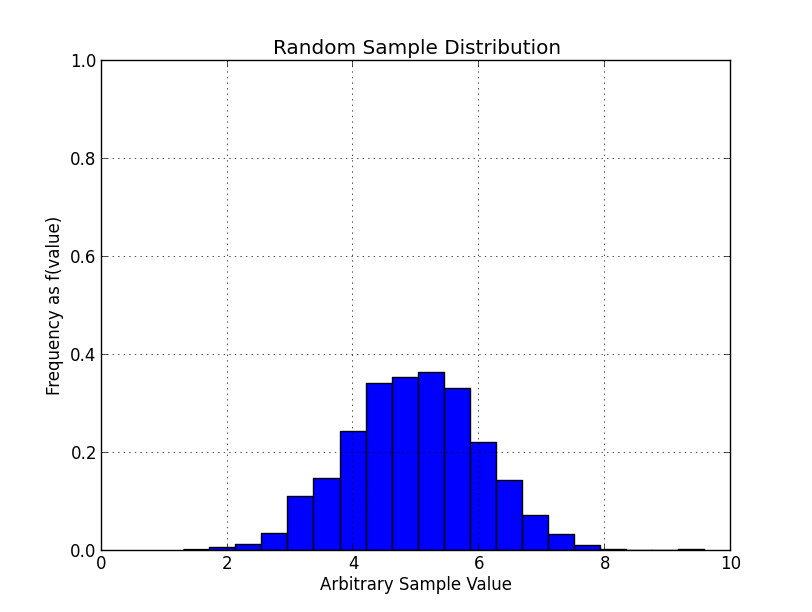
\includegraphics[width=.9\textwidth]{central_limit_1.png}
\caption{Random sampling converges to a Gaussian distribution as N
  increases; N = 1000.}
\end{figure}
Additionally, the standard deviation of the mean of the mean of N random
samples over many trials decrease with $sqrt{N}$. Each N value is trialed 1000 times.
\begin{figure}[H]
\centering
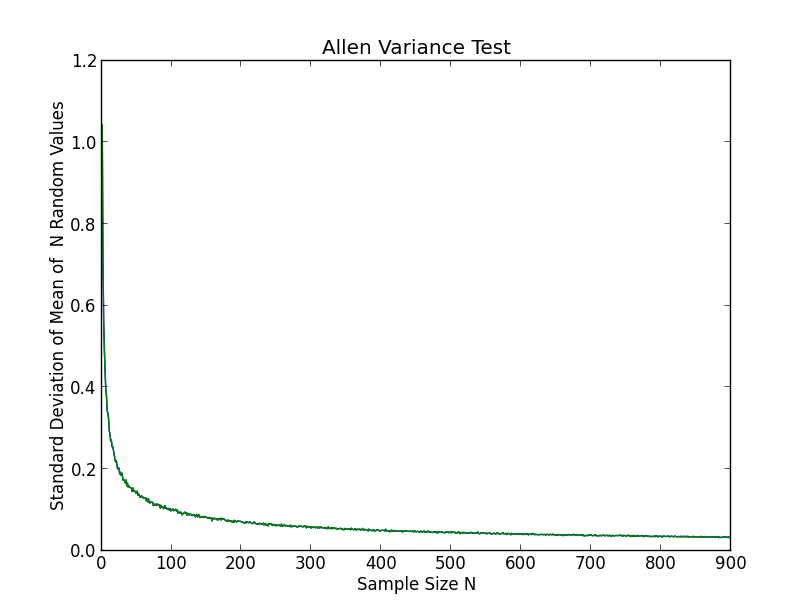
\includegraphics[width=.9\textwidth]{allen_variance_test.png}
\caption{The standard deviation of the mean of the mean over many trials
  of N random samples is plotted against N. There seems to be a
  $sqrt{N}$ relationship.}
\end{figure}
\section{Data and Results}
The results of the experiments are collected in this section.
\subsection{FM Radio Receiver}
\begin{figure}[H]
\centering
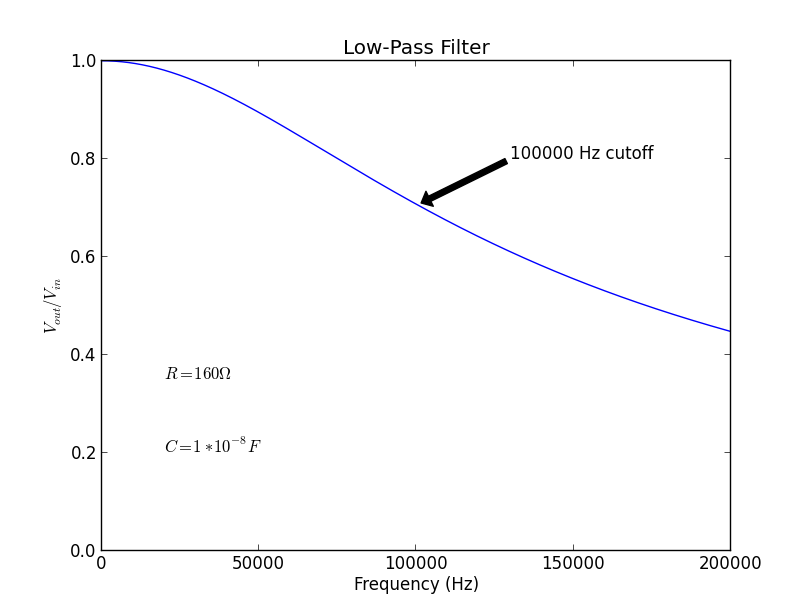
\includegraphics[width=.9\textwidth]{low_pass_filter.png}
\caption{The output of the radio receiver after FM Demodulation plotted
  against frequency.}
\end{figure}
For the given signal of 100 kHz, the values chosen for the resistor and
capacitor are $160\Omega$ and $1*10^{-8}$ to match the frequency. As
expected, the drop in voltage is steepest at the given cutoff
frequency. 
\section{Noise and Central Limit}
The thermal noise distribution follows the same math principles of
random distributions. The standard deviation of the mean of the mean of
N samples against N is given by Figure 5. For just the standard
deviation of the mean of N sample size, it is given by this figure:
\begin{figure}[H]
\centering
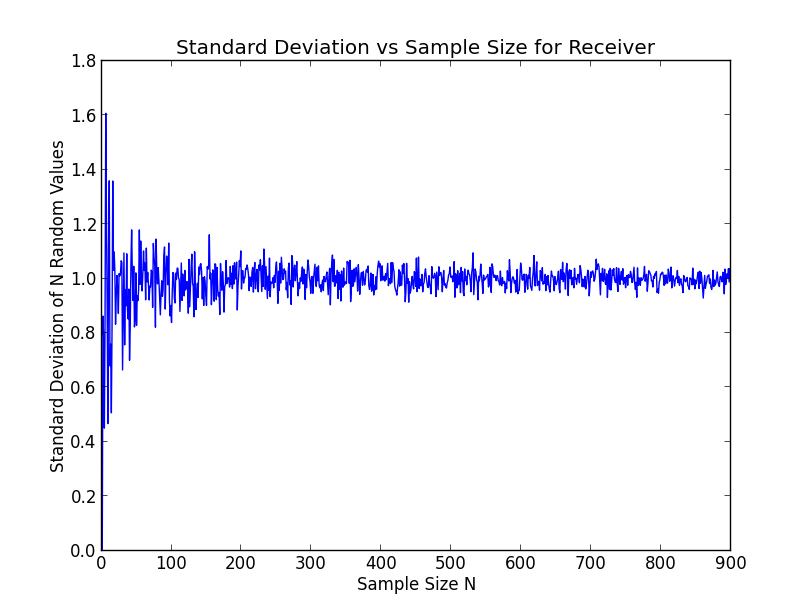
\includegraphics[width=.9\textwidth]{allen_2.png}
\caption{The standard deviation to the mean of N random samples is
  calculated just once for each N and is plotted against N}
\end{figure}
As expected, the graph follows some downward trend with increasing N but
it's not as clean as Figure 5 because each N is trialed only once.
\section{Discussion and Analysis}
The results and methods presented in the previous sections and discussed, analyzed,
and explained here.
\subsection{FM Radio Receiver}
As seen from the graph, 100000 Hz is the cutoff value of the filter once
the appropriate capacitor and resistor values are used. At frequencies
lower than 100000 Hz, the ratio of $V_{out}$ to $V_{in}$ is high; this
filter is to let low frequencies pass while filtering out high
frequencies. The ratio gets much lower past the cutoff frequency.
\subsection{Amplifier}
The amplifier is a complex circuit relative to the demodulator. The
values you choose for one part of the circuit can affect another part
since several values are connected by ratios to ensure that $V_{BE}$
remains constant at 0.7~ V. Fortunately, you can select which values to
begin with - whether that's the signal frequency or one of the
resistances. In the end, as long as the ratios are correct, the signal
should be correctly amplified.
\subsection{Noise}
Noise is everywhere. Although samples of noise phenomena can seem like
individual occurences, the Law of Large Numbers start to take effect and
present the true nature of the electrons. Noise can be undesired or
innocuous, depending on the nature of the experiment. In astronomy,
noise can come into the form of frustrating atmostpheric interference or in the form
of internal receiver signals of a telescope. Noise shows how the
universe disperses its seeds and the similar behaviors, on the fundamental
level, among many substances.
\subsection{Central Limit Theorem}
The central limit theorem makes powerful statements on the nature of our
universe. It shows that, fundamentally, math can model a wide range of
phenomena, even when you don't expect it to. Noise distribution is just
one of many examples of submission to this aspect of nature. Systems and occurances
sometimes behave statistically and it's not obvious - it's through
experimental observation that these concepts come into light. The
converging nature of the data really represents powerful mathematical statements.

\section{Conclusion}
The FM Demodulator and the amplifier served their purposes: they
received certain frequency signals and amplified incoming signals,
respectively. These constructions are basic models of the versions used
by companies for real-life products, but they present the underlying
principles in designing electronics and in manipulating electromagnetic
waves for specialized usage. The sensitive nature of electronics can be
challenging since precision is key; however, it is due to this nature
that electronics and circuits can be very diverse and unique. At their
deepest core, these systems still behave according to the mathematical
laws of the universe, as shown by the presence of Gaussian distributions
in even thermal noise. Ultimately, these systems converge to
fundamental, big picture concepts on both the small and large scales. In
radio astronomy, it would not be a surprise to encounter applicable
mathematical models during  real-time observations and appliance usage.

\end{document}
